\documentclass[12pt]{article}
\usepackage{amsfonts}
\usepackage{graphicx}

%%%%%%%%%%%%%%%%%%%%%%%%%%%%%%%%%%%%%%%%%%%%%%%%%%%%%%%%%%%%%%%%
%
% dimensions choisies par l'utilisateur (bricolage personnel)

\newdimen\decalage

\paperheight=29.7 true cm \paperwidth=21 true cm
\textheight=25.7 true cm \textwidth=17 true cm
\decalage=0 true cm

% déduction de \topmargin,
% \evensidemargin et \oddsidemargin

\oddsidemargin=\paperwidth
\advance\oddsidemargin by -\textwidth
\divide\oddsidemargin by 2
\advance\oddsidemargin by -1 in
\evensidemargin=\oddsidemargin
\advance\oddsidemargin by \decalage 
\advance\evensidemargin by -\decalage

\topmargin=\paperheight
\advance\topmargin by -\headheight
\advance\topmargin by -\headsep
\advance\topmargin by -\textheight
\advance\topmargin by -\footskip
\divide\topmargin by 2
\advance\topmargin by -1 in

%
%%%%%%%%%%%%%%%%%%%%%%%%%%%%%%%%%%%%%%%%%%%%%%%%%%%%%%%%%%%%%%%%

\begin{document}

\title{Compte rendu du TP6 et TP7 - Image}
\author{Louis Allain}
\maketitle

\section{Traitements de base}

\subsection{Acquérir une image}

Réponses aux question :
\begin{enumerate}

	\item 
		Acquérrir l'image.
		\begin{verbatim}
			chimp_img = io.imread('../res/chimpanze.jpg')
		\end{verbatim}
		
	\item
		Afficher l'image réelle.
		$$
			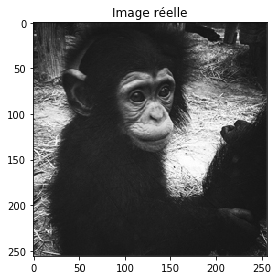
\includegraphics[width=0.3\textwidth]{img_reelle.png}
		$$
		
	\item
		Enregistrer un zoom de l'image sous une autre image.
		$$
			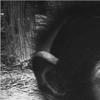
\includegraphics[width=0.3\textwidth]{chimpanze_zomm.jpg}
		$$
		
	\item
		Appliquer un masque sur l'image.
		
\end{enumerate}

\subsection{Echantillonnage}
	
Réponses aux question :
\begin{enumerate}

	\item 
		Acquérrir l'image de l'exo précédent.
		\begin{verbatim}
			chimp_img = io.imread('../res/chimpanze.jpg')
		\end{verbatim}
		
	\item
		Sous-échantillonner l'image : \\
		$$
			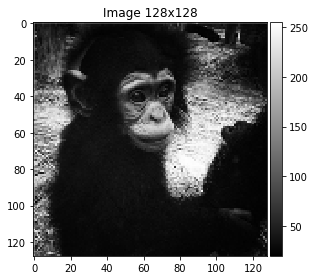
\includegraphics[width=0.3\textwidth]{res128.png}
			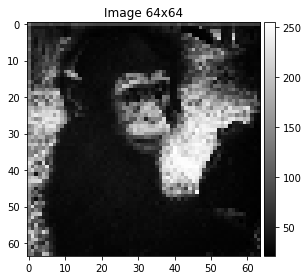
\includegraphics[width=0.3\textwidth]{res64.png}
		$$
		$$
			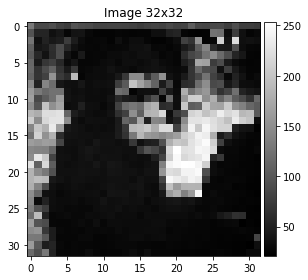
\includegraphics[width=0.3\textwidth]{res32.png}
			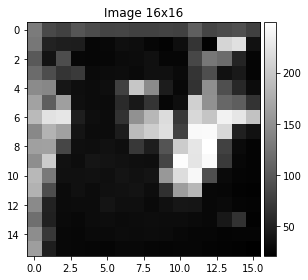
\includegraphics[width=0.3\textwidth]{res16.png}
		$$
		
	\item
		Fonction 'echantillonnage' : 
		\begin{verbatim}
			def echantillonnage(img, factor):
    
				ret = np.zeros(shape=(img.shape[0]//factor, img.shape[1]//factor))
				for i in range(0, img.shape[0], factor):
						
						for j in range(0, img.shape[1], factor):
								ret[i//factor][j//factor] = img[i][j]
				return ret
		\end{verbatim}
		
\end{enumerate}

\subsection{Histogramme}
	
Réponses aux question :
\begin{enumerate}

	\item 
		Fonction histogramme avec normalisation :
		\begin{verbatim}
			def histogramme(img, norme=1):
    
				ret = np.zeros(256)
				for i in range(0, img.shape[0]):
						for j in range(0, img.shape[1]):
								
								ret[img[i][j]] += 1
								
				# Normalise si besoin
				if(norme > 1):
						for i in range(0, ret.shape[0]):
								ret[i] = ret[i]/norme
								
				return ret
		\end{verbatim}
		
		Voici les histogrammes obtenus :
		$$
			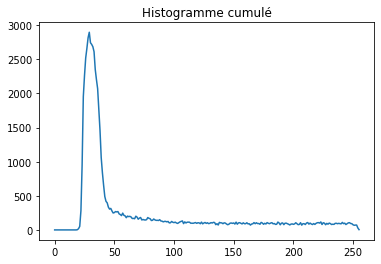
\includegraphics[width=0.3\textwidth]{hist_cumul.png}
			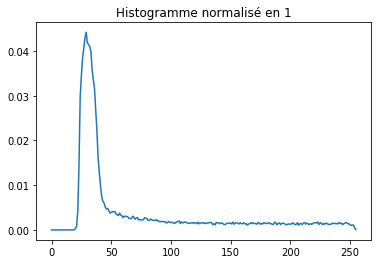
\includegraphics[width=0.3\textwidth]{hist_norm.png}
		$$
	
	\item
		Changement de contraste de l'image : 
		\begin{verbatim}
			chimp_img_3 = chimp_img_2
				h = histogramme(chimp_img_3, (256*256))
				for i in range(0, chimp_img_3.shape[0]):
								for j in range(0, chimp_img_3.shape[1]):
										chimp_img_3[i][j] = chimp_img_3[i][j] * h[chimp_img_3[i][j]]

		\end{verbatim}
		Voici l'image obtenue : 
		$$
			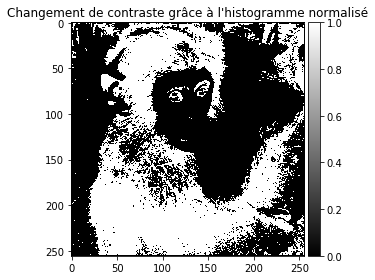
\includegraphics[width=0.3\textwidth]{chg_cont.png}
		$$
\end{enumerate}

\subsection{Convolution, détection de contour}
	
Réponses aux question :
\begin{enumerate}

	\item 
		Appliquer un filtre de détection de contour : 
		$$
			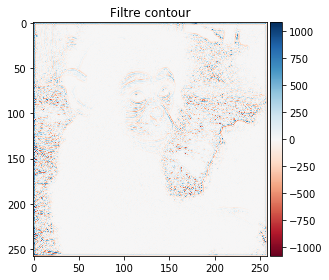
\includegraphics[width=0.3\textwidth]{filtre_cont.png}
		$$
		
	\item
		Appliquer un filtre gaussien : 
		$$
			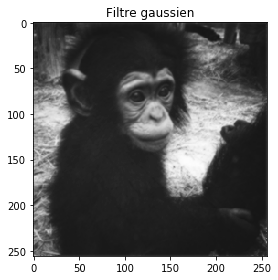
\includegraphics[width=0.3\textwidth]{filtre_gauss.png}
		$$
		
	\item
		Fonction 'convolution' : 
		\begin{verbatim}
			def convolution(img, Mc):
    
				xMc = int((Mc.shape[1]-1)/2)
				yMc = int((Mc.shape[0]-1)/2)
				imgCp = img
				m = int(img.shape[1] - xMc)
				
				for i in range(xMc, m):
						for j in range(yMc, img.shape[0]-yMc):
								acc = 0.0
								for k in range(-xMc, xMc+1):
										for l in range(-yMc, yMc+1):
												acc = acc + img[j+l][i+k]*Mc[l+yMc][k+xMc]
								imgCp[j][i] = acc
				return imgCp
		\end{verbatim}
		
\end{enumerate}

\subsection{Filtre moyenneur}
	
Réponses aux question :
\begin{enumerate}

	\item 
		Acquérir une image en nuance de gris : 
		\begin{verbatim}
			fleur = io.imread('../res/fleur.jpg') 
		\end{verbatim}
	\item
		Appliquer un filtre moyenneur : 
		$$
			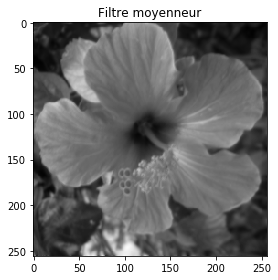
\includegraphics[width=0.3\textwidth]{filtre_moy.png}
		$$
		
	\item
		Le filtre précédent floute l'image, il agit comme un filtre passe bas.
		
\end{enumerate}

\section{Traitement de l'image et transformée de Fourier}

\subsection{Transformée de Fourier}

Réponses aux question :
\begin{enumerate}
	
	\item 
		Je choisis d'utiliser cette image pour la suite : 
		$$
			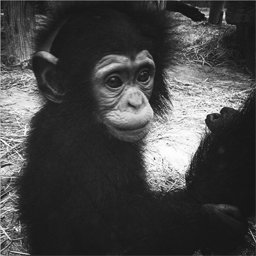
\includegraphics[width=0.3\textwidth]{chimpanze.jpg}
		$$
	
	\item 
		Affichage de la phase et de l'amplitude de l'image avec fft2 : 
		$$
			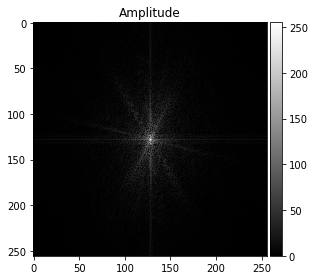
\includegraphics[width=0.3\textwidth]{img_amp.png}
			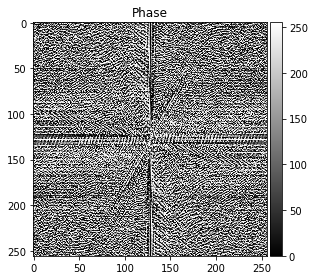
\includegraphics[width=0.3\textwidth]{img_phase.png}
		$$
		
	\item
		Retrouver la phase et l'amplitude avec ifft2 
		$$
			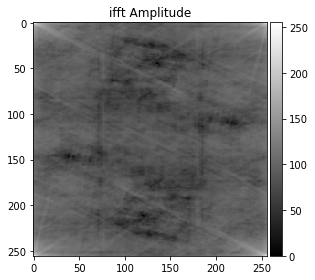
\includegraphics[width=0.3\textwidth]{ifft_amp.png}
			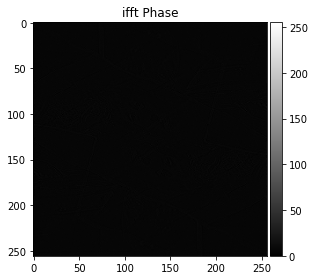
\includegraphics[width=0.3\textwidth]{ifft_phase.png}
		$$
		
\end{enumerate}

\subsection{Filtrage par convolution}

Réponses aux question :
\begin{enumerate}
	
	\item 
		Je choisis d'utiliser cette image pour la suite : 
		$$
			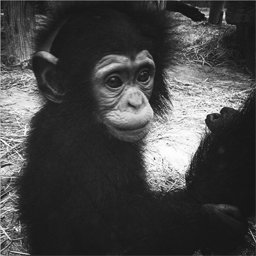
\includegraphics[width=0.3\textwidth]{chimpanze.jpg}
		$$
	
	\item 
		Application du filtre passe bas par convolution, code : 
		\begin{verbatim}
			Mpb = np.array([
				[1, 3, 1],
				[3, 5, 3],
				[1, 3, 1]])
			convolution(chimp, Mpb)
		\end{verbatim}
	\item
		Résultat du filtre précédent : 
		$$
			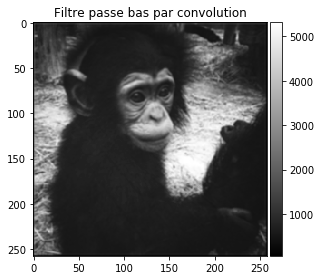
\includegraphics[width=0.3\textwidth]{fil_pb_conv.png}
		$$
	\item
		Résultat du filtre passe haut par convolution : 
		$$
			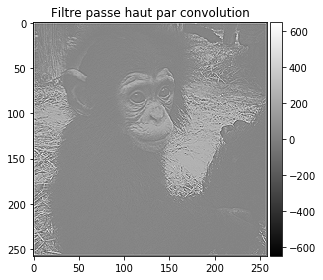
\includegraphics[width=0.3\textwidth]{fil_ph_conv.png}
		$$
		
\end{enumerate}

\subsection{Filtrage par transformée de Fourier}

Réponses aux question :
\begin{enumerate}
	
	\item
		Résultat du filtre passe bas par tranformée de Fourier : 
		$$
			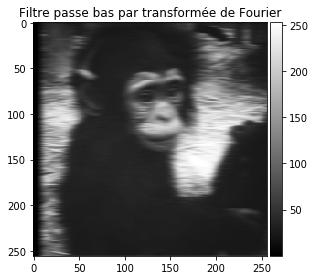
\includegraphics[width=0.3\textwidth]{fil_pb_fou.png}
		$$
	\item
		Résultat du filtre passe haut par tranformée de Fourier : 
		$$
			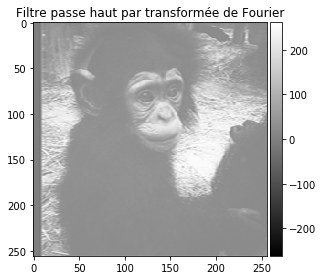
\includegraphics[width=0.3\textwidth]{fil_ph_fou.png}
		$$
		
\end{enumerate}

\end{document}